\documentclass[a4paper, 11pt]{scrartcl}
\usepackage[top = 2.5cm, bottom = 2cm, left = 2.5cm, right = 2.5cm]{geometry}
\usepackage[onehalfspacing]{setspace}
\usepackage{mathtools}
\usepackage{fontspec}
\usepackage[english]{babel}
\usepackage{hyperref}
\usepackage{environ}
\hypersetup{
	colorlinks = true,
	linkcolor  = black,
	citecolor  = blue,
	urlcolor   = blue
}
\usepackage{graphicx}
\usepackage{acronym}
\usepackage{enumerate}
\usepackage{enumitem}
\usepackage{tabularx}
\usepackage{booktabs}
\usepackage{multirow}
\usepackage{float}

\usepackage{sourcecodepro}
\usepackage{listings}
\usepackage{xcolor}

\definecolor{codegreen}{rgb}{0,0.6,0}
\definecolor{codegray}{rgb}{0.5,0.5,0.5}
\definecolor{codepurple}{rgb}{0.58,0,0.82}
\definecolor{backcolour}{rgb}{0.95,0.95,0.92}

\lstdefinestyle{mycodestyle}{
	backgroundcolor = \color{backcolour},   
	commentstyle = \color{codegreen},
	keywordstyle = \color{magenta},
	numberstyle = \tiny\color{codegray},
	stringstyle = \color{codepurple},
	basicstyle = \ttfamily\footnotesize,
	breakatwhitespace = false,         
	breaklines = true,                 
	captionpos = b,                    
	keepspaces = true,                 
	numbers = left,                    
	numbersep = 5pt,                  
	showspaces = false,                
	showstringspaces = false,
	showtabs = false,                  
	tabsize = 2
}

\lstset{style = mycodestyle}

\lstnewenvironment{code}{\lstset{language = Java, basicstyle = \ttfamily\small, backgroundcolor = \color{backcolour}}}{}
\newcommand{\inlinecode}[1]{\texttt{\small #1}}
\NewEnviron{hiddencode}{}

\usepackage{csquotes}
\usepackage[backend = biber, style = apa]{biblatex}
\addbibresource{../iris_literature.bib}

\setlength{\parskip}{1em}

\title{IRIS - ODD Protocol}
\author{}
\date{\today}

\begin{document}

\maketitle
\tableofcontents

\newpage
\listoffigures
\listoftables

\section*{List of Acronyms}
\begin{acronym}
\acro{ECS}{Entity Component System}
\acro{GCM}{Global Change Model}
\acro{GERICS}{The Climate Service Center Germany}
\acro{IRIS}{Ixodes RIcinus Simulator}
\acro{ODD}{Overview, Design Concepts and Details}
\acro{RCM}{Regional Change Model}
\end{acronym}


\newpage
\section{Overview}
In this document, we describe the model IRIS (Ixodes RIcinus Simulator). It is a cohort-based and spatially-explicit population model to simulate local dynamics of \textit{Ixodes ricinus} ticks under climate change. It consists of behavioural rules of \textit{I. ricinus} ticks and takes weather and climate data as input to simulate the seasonal spatio-temporal abundance and questing activity of ticks of different life stages over a year with daily time steps. Thereby, the emphasis is put on nymphal ticks, as they pose the greatest risk to humans. The model dynamic is driven by the population's response to prevailing temperatures and relative humidity as well as habitat conditions in each time step.

This model description follows the Overview, Design concepts and Details (ODD) protocol. ODD is a standard format to systematically describe models in a comprehensive and transparent way aiming to allow for model replication ~\parencite{Grimm.2010, Grimm.2020}.


\subsection{Purpose}
The overall purpose of the IRIS model is to understand the impact of climate change on the spatial and temporal abundance of \textit{I. ricinus} ticks on the local scale. As nymphal ticks are highly relevant vectors of Lyme borreliosis, it is important to gain a better understanding of their future climate-dependent dynamics to assess the exposure risk for humans. 


\subsection{Entities, state variables and scales}

\subsubsection{Entities}
The model is composed of grid cell entities.

\subsubsection{State variables}
By implementing IRIS using an Entity Component System (ECS) framework, the state variables of the model are organised in so-called \textit{components}, which are attached to the grid cell entities. Table \ref{tab:state_variables} provides an overview of the state variables of the IRIS model.

\begin{table}[H]
\caption{State variables of the IRIS model.}
\label{tab:state_variables}
\begin{tabularx}{\textwidth}{lllll}
\toprule
\textbf{Component} & \textbf{Variable} & \textbf{Type} & \textbf{Default} & \textbf{Description} \\
\midrule
\multirow{2}{*}{Position} 	 & x  				& int  		& null & x coordinate \\
							 & y    			& int  		& null & y coordinate \\
Habitat 				  	 & type 			& enum Type & null & Habitat type \\
TickAbundance 			  	 & stage 			& enum LifeCycleStage  & null & Tick cohort \\
\multirow{3}{*}{Temperature} & meanTemperature  & double  	& null & Mean temperature \\
							 & minTemperature   & double  	& null & Minimum temperature \\
							 & maxTemperature   & double  	& null & Maximum temperature \\
Humidity 					 & relativeHumidity & double  	& null & Relative humidity \\
\bottomrule
\end{tabularx}
\end{table}

In addition, each grid cell entity is provided with a unique identification number used for internal processing by the ECS framework. This \inlinecode{entityID} is linked to the component \inlinecode{Position} within the ECS resource {SpatialIndex} using a HashMap. The state variables \inlinecode{type} and \inlinecode{stage} of the components \inlinecode{Habitat} and \inlinecode{TickAbundance} are specified by enumerations. The enumeration \inlinecode{Type} specifies the habitat type. It can take the following values:
\begin{small}
\begin{itemize}[noitemsep]
	\item FOREST, ECOTONE, MEADOW
\end{itemize}
\end{small}

The enumeration \inlinecode{LifeCycleStage} specifies the tick cohort. It can take the following values:
\begin{small}
\begin{itemize}[noitemsep]
	\item LARVAE, NYMPH, ADULT,  
	\item LARVAE\_INACTIVE, NYMPH\_INACTIVE, ADULT\_INACTIVE
	\item LARVAE\_ENGORGED, NYMPH\_ENGORGED, ADULT\_ENGORGED
	\item LARVAE\_LATE\_ENGORGED, NYMPHS\_LATE\_ENGORGED
\end{itemize}
\end{small}


\subsubsection{Scales}
The spatial scale of the model corresponds to a local region of approximately $14400 \mathrm{m}^{2}$ ($= 0.0144 \mathrm{km}^{2}$). The model landscape consists of $12 \times 12 = 144$ grid cells. A grid cell corresponds to an area of $10 \mathrm{m} \times 10 \mathrm{m} = 100 \mathrm{m}^{2}$. The reason for this is that tick densities are usually expressed in numbers per $100 \mathrm{m}^{2}$ ~\parencite[see e.g.][Table 2]{Boehnke.2015}. This is because the standard method of collecting host-seeking ticks (called flagging) is typically done over a sampling area of $100 \mathrm{m}^{2}$ ~\parencite{Brugger.2016, Schulz.2014}.

A single simulation run of IRIS covers a period of one year with daily time steps. On this time scale, we are able to capture the local population dynamics of ticks well. Since our model is cohort-based we are looking at averaged behaviour which harmonises well with daily time steps. Required input data such as temperature and humidity is available on a daily basis from German weather stations and climate simulation models (see Section ~\ref{input_data} for details). Furthermore, daily time steps are also computationally feasible.


\subsection{Process overview and scheduling}
The IRIS model simulates one year from January 1 to December 31 and is executed in daily discrete time steps. A leap year also includes 29 February. In each time step, the following model processes are executed for every grid cell and the state-variables are updated in the following order:

\begin{enumerate}[noitemsep]
	\item Weather
	\item Activity
	\item Feeding
	\item Development
	\item Freezing
	\item Desiccation
\end{enumerate}

The process \inlinecode{Weather} is responsible for setting the daily temperature and relative humidity and updates the state variables \inlinecode{meanTemperature}, \inlinecode{minTemperature}, \inlinecode{maxTemperature} and \inlinecode{relativeHumidity}. The process \inlinecode{Activity} involves the active search for a host (also known as \textit{questing}) or putting ticks into a state of inactivity. The process \inlinecode{Feeding} controls the feeding success of ticks, ~i.e.\ the successful attachment of a ticks to a hosts. Furthermore, it includes a translocation process by which ticks are moved to other locations on the model landscape, ~i.e.\ moved to a cohort in another grid cell. The process \inlinecode{Development} involves the transition from one life cycle stage to the next. The processes \inlinecode{Freezing} and \inlinecode{Desiccation} control tick mortality in case of unfavourable environmental conditions. All processes (except for \inlinecode{Weather}) update the state variable \inlinecode{stage} of each grid cell. Each process is described in more detail in Section~\ref{submodels}. A visualisation of the scheduling process is displayed in Figure~\ref{fig:iris_scheduling}.

The multi-year life cycle of the modelled ticks is captured indirectly. This is done by assigning a certain number of ticks at the beginning of a simulation run, so that each life cycle stage is represented in the model through its respective cohort.

\begin{figure}[h!]
\centering
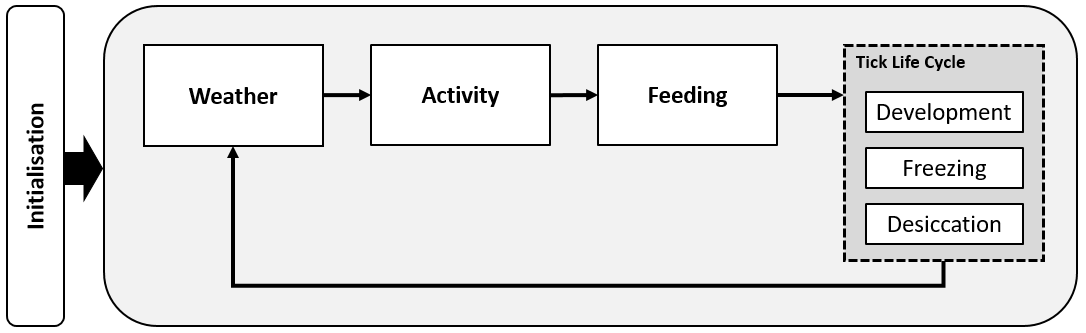
\includegraphics[width=0.8\linewidth]{scheduling}
\caption{Overview over the scheduling of model processes}
\label{fig:iris_scheduling}
\end{figure}


\newpage
\section{Design Concepts}\label{design_concepts}
\textbf{Basic principles:} IRIS is a spatially explicit stochastic cohort-based tick population model. It is composed of grid cells with sub populations of \textit{I. ricinus} ticks belonging to a cohort. Each cohort represents a tick life cycle stage together with a behavioural state. Three tick life cycle stages are possible: (1) \emph{larvae}, (2) \emph{nymphs} and (3) \emph{adults}. Furthermore, each life cycle stage can adopt one of four behavioural states: (i) \emph{questing}, (ii) \emph{inactive}, (iii)  \emph{engorged} and (iv) \emph{late engorged}. The latter is a special case of the behavioural state \emph{engorged} which applies only to larvae and nymphs (see section \ref{feeding} for details). Hence, in total there are 11 tick cohorts present in the model. Technically, these cohorts exist in every cell of the model landscape, e.g. active nymphs in grid cell $(0,0)$ belong to a different cohort than active nymphs in grid cell $(3,5)$. However, for model evaluations the cohorts are considered in total. The grid cells form a model landscape that serves as habitat for \emph{I. ricinus} sub populations. Three different idealised habitat types exist in the model: (a) \emph{forest}, (b) \emph{ecotone} and (c) \emph{meadow}. Daily temperature and relative humidity influence the behaviour of the modelled ticks and thereby drive the model dynamics. With the input of future weather data from climate simulations, the model is able to simulate the expected future abundance of ticks. A visualisation of the model landscape with habitat types and tick cohorts is displayed in Figure~\ref{fig:iris_landscape}.

\begin{figure}[h!]
\centering
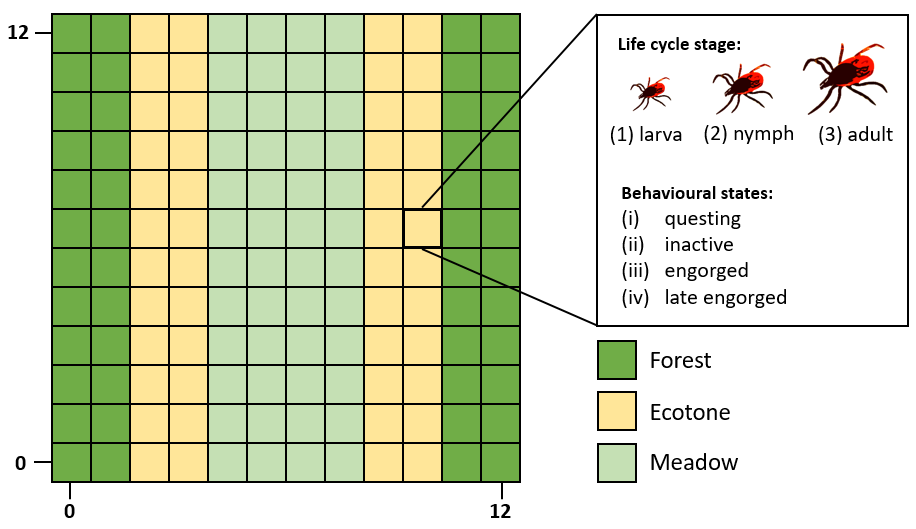
\includegraphics[width=0.75\linewidth]{landscape}
\caption{The IRIS model landscape consists of 12 x 12 grid cells. The colour of each grid cell indicates the habitat type: forest (dark green), ecotone (light brown) and meadow (light green). Each cell contains tick cohorts consisting of one of 3 life cycle stages (larva, nymph, adult) together with one of 4 behavioural states (questing, inactive, engorged and late engorged).}
\label{fig:iris_landscape}
\end{figure}

IRIS was implemented in Java using version 2.3.0 of the Artemis-odb Entity-Component-System (ECS) framework\footnote{\url{https://github.com/junkdog/artemis-odb}}.


\textbf{Emergence:} The main output of the model are numbers of \emph{I. ricinus} ticks in each of the 11 cohorts, with the cohort of active nymphs being the most important. The numbers in each cohort emerge from the interaction of environmental conditions in each grid cell which is influenced by the weather and behavioural rules of ticks.

\textbf{Adaptation:}

\textbf{Sensing:}

\textbf{Stochasticity:} To determine random numbers we use the seedable random number generator ``Mersenne-Twister'' provided by Apache Commons Math library (version 3.6.1.). In addition we implemented a method \inlinecode{roundRandom()} to allow processes that statistically affect less than a single tick to still happen.

\begin{lstlisting}[language = Java, caption = {Overview of roundRandom() method}]
public int roundRandom(float value) {
	int base = (int) value;
	float remainder = value - base;
	
	if (remainder == 0) {
		return base;
	}
	if (random() < remainder) {
		return base + 1;
	}
	return base;
}
\end{lstlisting}


\textbf{Collectives:} Since this model is cohort-based, all of the eleven model cohorts can be interpreted as collectives that combine a subpopulation of a certain number of \emph{I. ricinus} ticks in each grid cell. Interaction between cohorts of different grid cells take place via the translocation process implemented in the \inlinecode{Feeding} component (see Section~\ref{feeding} for details)

\textbf{Observation:}



\newpage


\section{Details}

\subsection{Globals}

\subsection{Initialisation}\label{initialisation}
The initialisation of the model involves the following steps. First, IRIS is started by calling the main method of one of the classes in the project folder `experiments`. The class \inlinecode{AdHoc} can be called to simulate a single year. It is also possible to pass individual simulation parameters to the \inlinecode{AdHoc} class. The other two classes (\inlinecode{SensitivityAnalysis}, \inlinecode{SensitivityAnalysisLN}) in the `experiments' folder are used to carry out sensitivity analyses. The simulation parameters are already defined there within these classes.

When calling the main method of the class \inlinecode{AdHoc} individual command line parameters, if available, are first passed to the model (see Table~\ref{tab:initialisation_parameters}). These parameters are used to call the method \inlinecode{run()} in the class \inlinecode{Model}. These include, among other items, the initial number of larvae, nymphs and adults.

\begin{table}[h!]
\caption{Input parameters}
\label{tab:initialisation_parameters}
\begin{tabularx}{\textwidth}{lllll}
\toprule
\textbf{Parameter} 	& \textbf{Symbol} & \textbf{Default value} & \textbf{Type} & \textbf{Description} \\
\midrule
seed    			&   & 42    & int     & random seed \\
weather     		& - & -     & String  & path to weather input file \\
output     			& - & -     & String  & path to set directory of output files \\
initialLarvae       &   & 150   & int     & initial number of inactive larvae \\
initialNymphs       &   & 150   & int     & initial number of inactive nymphs \\
initialAdults       &   & 150   & int     & initial number of inactive adults \\
activationRate      &   & 0.02  & float   & activation rate  \\
summary       		&   & true & boolean & write only summary outputs \\
\bottomrule
\end{tabularx}
\end{table}

Afterwards, the random number generator is initialised with a random seed and the world configuration of the Entity Component System is assembled. This includes the registration of the ECS Systems (Activity, Feeding, TickLifeCycle, Weather) and Resources (Parameters, Randomness, SpatialIndex and TimeStep). This is followed by the initialisation of the model landscape, i.e.\ each grid cell is assigned a position $(x, y)$ and a habitat type (forest, ecotone, meadow). In addition, the ECS components (Habitat, Humidity, Position, Precipitation, Temperature, TickAbundance) are added to the grid cells (i.e.\ the ECS entities).

\subsubsection{Adjusting the initial number of larvae using beech mast fructification data}\label{subsubsec:initial_larvae_with_beech_mast}
If data is available the model is able to use beech mast fructification data of the European beech \textit{Fagus sylvatica} to adjust the initial number of larvae at the beginning of a simulation run. This reason for this adjustment can be explained as follows: Small rodents serve as host animals especially for \textit{Ixodes ricinus} larvae~\parencite{Cayol.2017}. A higher density of small rodents in a given year causes an increase in the population of larvae and nymphs in the following year~\parencite{Brugger.2018}. Data on beech mast can be used to estimate rodent populations, because a year with high mast production leads to an increase in the rodent population in the following year due to higher food supply~\parencite{Clement.2009}. Hence, we assume that the initial number of larvae at the beginning of a simulation run of a given year is influenced by the beech mast two years before.

The type of beech mast is divided into four classes and given as an index. Based on this fructification index, the model adjusts the initial number of larvae at the beginning of a simulation run. The default number of initial larvae is reduced if when the second year before the simulated year is not a mast year with full fructification. The strength of the reduction depends on the type of beech mast, i.e.\ the fructification index. Table~\ref{tab:fructification_adjustment} gives an overview over the adjustment values. Information on the beech mast input data can be found in Section~\ref{subsubsec:beech_mast_data}.

\begin{table}[h!]
\caption{Adjustment of initial number of larvae based on the fructification index}
\label{tab:fructification_adjustment}
\begin{tabularx}{\textwidth}{clll}
\toprule
\textbf{Fructification index} & \textbf{Description}    & \textbf{Adjustment Value} & \textbf{Reference} \\
\midrule
1				 	  		  & absent fructification 	& 	0.25 & own estimation \\
2 				 	  		  & scarce fructification	&	0.5	& own estimation  \\
3 					  		  & common fructification	& 	0.75 & own estimation \\
4					 		  & full fructification 	& 	1.0	& own estimation \\
\bottomrule
\end{tabularx}
\end{table}

\subsection{Input data}\label{input_data}
IRIS uses observed weather and simulated climate data and optionally data on beech mast as input data. In detail, the model requires the following input data on a daily basis:

\begin{itemize}[noitemsep]
\item Daily mean near-surface air temperature [°C]
\item Daily Maximum Near-Surface Air Temperature [°C]
\item Daily Maximum Near-Surface Air Temperature [°C]
\item Daily near surface relative humidity [\%]
\end{itemize}

An overview over the input parameters can be found in Table ~\ref{tab:input_parameters}.

\subsubsection{Observed weather data}
Observed daily temperature and humidity data from the Deutscher Wetterdienst (DWD) was included in the model both for model calibration and simulation of past years~\footnote{\url{https://www.dwd.de/DE/leistungen/klimadatendeutschland/klimadatendeutschland.html}}. In particular, the following data was used from the weather station in Regensburg (Station ID: 4104; Location: 49° 02', 12° 06'):

\begin{itemize}[noitemsep]
	\item Daily mean of temperature (TMK, [°C])
	\item Daily minimum of air temperature at 2 m height (TNK, [°C])
	\item Daily maximum Of air temperature at 2 m height (TXK, [°C])
	\item Daily mean of relative humidity (UPM, [\%])
\end{itemize}

Since the weather station in Regensburg is located at an altitude of 365 metres, but the sampling site in Haselmühl or which the model calibration and simulations were carried out is located at a higher altitude of 430 metres, the temperature values from the DWD data set were adjusted by according to the dry-adiabatic temperature gradient. Specifically, the values were reduced by $-0.64 = (430 - 365) / 100 \times -0.98$.

This adjustment must always be made individually for each location for which simulations are to be carried out whenever its altitude differs substantially from the altitude of the location of the measurement of temperatures.

\subsubsection{Climate simulation data}
Climate simulation data was provided by The Climate Service Center Germany (GERICS). A total of 15 combinations of Global Change Models (GCMs) and Regional Chance Models (RCMs) were provided for the RCP8.5 scenario, i.e.\ the scenario that exceeds 4K global warming (see Table ~\ref{tab:climate_models} for an overview).

Bias-adjusted EURO-CORDEX simulations were provided for the following parameters:
\begin{itemize}[noitemsep]
\item Bias Adjusted Near-Surface Air Temperature (tas, [K])
\item Bias Adjusted Daily Maximum Near-Surface Air Temperature (tasmax, [K])
\item Bias Adjusted Daily Minimum Near-Surface Air Temperature (tasmin, [K])
\end{itemize}

Homogenised EURO-CORDEX simulations were provided for the following parameter:
\begin{itemize}
\item Near-Surface Relative Humidity (hurs, [\%])
\end{itemize}
% noch etwas mehr erläutern (EURO-CORDEX, bias-adjusted, homogenised, etc., Warum so viele Modelle)


\begin{table}[h!]
\caption{13 GCM-RCM combinations for the RCP8.5 scenario}
\label{tab:climate_models}
\begin{tabularx}{\textwidth}{ll}
\toprule
\textbf{Driving GCM and realisation}  & \textbf{Downscaling RCM} 	\\
\midrule
CanESM2; r1i1p1 				 	  & CCLM4-8-17; v1  		 	\\
CanESM2; r1i1p1 				 	  & REMO2015; v1 				\\
HadGEM2-ES; r1i1p1 					  & Aladin63; v1 				\\
HadGEM2-ES; r1i1p1 					  & HadREM3; v1 				\\
HadGEM2-ES; r1i1p1 					  & HIRHAM5; v2 				\\
HadGEM2-ES; r1i1p1 					  & RACMO22E; v2 				\\
HadGEM2-ES; r1i1p1 					  & RCA4; v1 					\\
HadGEM2-ES; r1i1p1 					  & RegCM4-6; v1 				\\
HadGEM2-ES; r1i1p1 					  & REMO2015; v1 				\\
IPSL-CM5A-MR; r1i1p1 				  & RCA4; v1 					\\
IPSL-CM5A-MR; r1i1p1 				  & WRF381P; v1 				\\
MPI-ESM-LR; r3i1p1 					  & RCA4; v1 					\\
MPI-ESM-LR; r3i1p1 					  & REMO2015; v1				\\
\bottomrule
\end{tabularx}
\end{table}

% (Tests und Validierung hauptsächlich mit MPI-ESM-LR; r3i1p1, REMO2015; v1)
% erklären: als NetCDF file für Ausschnitt ca. Deutschland bekommen --> *.csv file (Rausziehen der Wetterzeitreihe mittels Skript)
% Umrechnung von K in Celsius

\subsubsection{Beech mast fructification data}\label{subsubsec:beech_mast_data}
IRIS is able to use beech mast fructification data of the European beech \textit{Fagus sylvatica}. This data can be used to adjust the initial number of larvae (for details see Section~\ref{subsubsec:initial_larvae_with_beech_mast}). Beech mast fructification data is given as an annual index. For the validation of the model we have used the values from~\cite{Brugger.2018}. A larger data set with fructification data between 1954 an 2016 is available from~\cite{Konnert.2016}.


\begin{table}[h!]
\caption{Input parameters}
\label{tab:input_parameters}
\begin{tabularx}{\textwidth}{llll}
\toprule
\textbf{Parameter} & \textbf{Symbol} & \textbf{Type}     & \textbf{Description}       \\
\midrule
meanTemperature    & $t_{mean}$      & double            & Daily mean temperature     \\
minTemperature     & $t_{\min}$      & double            & Daily max temperature      \\
maxTemperature     & $t_{\max}$      & double            & Daily min temperature      \\
humidity           & $h$             & double            & Daily humidity             \\
\midrule
fructificationIndex & $f$            & int               & Fructification index		  \\
\bottomrule
\end{tabularx}
\end{table}


\newpage
\subsection{Submodels}\label{submodels}

\subsubsection{Development}
This sub model is responsible for the development from one tick life cycle stage to the next. It is implemented in the method \inlinecode{development()} in the class \inlinecode{TickLifeCycle}. The life cycle of \textit{Ixodes ricinus} ticks consists of four life stages: eggs, larvae, nymphs, adults. Once the eggs have hatched into larvae, each further life cycle stage requires a bloodmeal to develop to the next life cycle stage~\parencite{tba}.

The development from one life cycle stage to the next takes place over specific periods of time. The development period begins at the beginning of July and ends either in early or mid-October, depending on the life cycle stage~\parencite{tba}. Since only engorged ticks can develop to the next life cycle stage, their number is subtracted from the respective cohort with behavioural state 'engorged' and added to the cohort of the next life cycle stage with behavioural state 'inactive'. We assume that all engorged ticks will have developed at the end of the development period:

\begin{equation}
n_{\text{developing}}(t) = \text{roundRandom}(\frac{n_{engorged}(t)}{t_{\text{end} - t_{\text{current}}}})
\end{equation}

The values of the start and end times of the development period are implemented as constants. Table ~\ref{tab:development_parameters} gives an overview over the development parameters.

The oviposition of adult ticks is not modelled explicitly. Hence, we assume that adult ticks become new larvae.
% need further explanation

\begin{table}[h!]
\caption{Time period of development to next life cycle stage}
\label{tab:development_parameters}
\begin{tabularx}{\textwidth}{lclcl}
\toprule
\textbf{Time period} 	& \textbf{Time step} & \textbf{Parameter Name}							& \textbf{Type}    & \textbf{Reference} \\
\midrule
Early July   			& 181   			 & \tiny{BEGIN\_OF\_DEVELOPMENT}					& int      & \cite{tba}   		\\
Mid-October     		& 289      			 & \tiny{END\_OF\_DEVELOPMENT\_LARVAE\_TO\_NYMPHS}	& int      & \cite{tba}      	\\
Early October    		& 274    			 & \tiny{END\_OF\_DEVELOPMENT\_NYMPHS\_TO\_ADULTS}	& int      & \cite{tba}     	\\
Mid-October     		& 289      			 & \tiny{END\_OF\_DEVELOPMENT\_ADULTS\_TO\_LARVAE}	& int      & \cite{tba}			\\
\bottomrule
\end{tabularx}
\end{table}

\subsubsection{Desiccation}
This sub model controls the desiccation of ticks. It is implemented in the method \inlinecode{desiccation()} in the class \inlinecode{TickLifeCycle}. In general ticks need at least 80 \% relative humidity in their local environment to survive ~\parencite{Medlock.2013, Gray.2016, Hauser.2018}. When the relative humidity falls below this level off-host ticks start to dry out and will eventually die unless the relative humidity rises again. Survival at lower relative humidity is possible but also requires lower temperatures ~\parencite{Ostfeld.2015}. Due to the favourable microclimatic conditions, ticks prefer woodland habitats and have a higher abundance there than for example in meadows ~\parencite{Lindstrom.2003, Boehnke.2015}.

At each time step this sub model checks the relative humidity and temperature. If these exceed certain thresholds a proportion of all questing ticks that are in such a grid cell will desiccate (see Table ~\ref{tab:desiccation_parameters}). The exact desiccation rate depends on the habitat type of the grid cell. Thereby we capture the favourable effect of the more humid microclimate within a forest compared to a meadow on tick survival. Desiccated ticks are removed from the modelled population.

\begin{table}[h!]
\caption{Habitat dependent desiccation rates and threshold values}
\label{tab:desiccation_parameters}
\begin{tabularx}{\textwidth}{llccl}
\toprule
\textbf{Parameter}							& \textbf{Habitat}  & \textbf{Value} & \textbf{Unit}	& \textbf{Reference} \\
\midrule
\multirow{3}{*}{\tiny{DESICCATION\_MINIMAL\_HUMIDITY}} 	& \multirow{3}{*}{-} & \multirow{3}{*}{80.0} & \multirow{3}{*}{\%} &  \cite{Medlock.2013} \\
													   	& 					 & 						 &					   &  \cite{Gray.2016}	\\
														& 					 & 						 &					   &  \cite{Hauser.2018} \\
\tiny{DESICCATION\_MINIMAL\_MEAN\_TEMP} 	& -    			 		 &   15.0  & °C  &  \cite{Ostfeld.2015} \\
\multirow{3}{*}{\tiny{DESICCATION\_RATE}}  	& Forest       			 &   0.02  & 1/day 	& own estimation \\
				 							& Ecotone 				 &   0.05  & 1/day  & own estimation \\
				 							& Meadow    			 &   0.10  & 1/day  & own estimation \\
\bottomrule
\end{tabularx}
\end{table}

\subsubsection{Freezing}
The sub model `freezing' is responsible for modeling the effect of extreme cold on ticks. It is implemented in the method \inlinecode{freezing()} in the class \inlinecode{TickLifeCycle}.

Ixodes ricinus ticks are quite resistant to low temperatures ~\parencite{Gray.2009}. But they can die when exposed to extreme cold with temperatures lower than approximately minus 15 degrees Celsius ~\parencite{Ostfeld.2015}. Especially without protective snow cover ticks can die of freezing under these conditions ~\parencite{Jore.2014}.

At each time step the sub model checks whether the minimum temperature $t_{\min}$ is below a threshold value of minus 18.9 degree Celsius. If that is the case, some of the ticks are considered dead and are hence removed from the modelled population. Table ~\ref{tab:freezing_parameters} contains the parameters that belong to the freezing sub model.

\begin{table}[h!]
\caption{Parameters of the freezing sub model}
\label{tab:freezing_parameters}
\begin{tabularx}{\textwidth}{lccl}
\toprule
\textbf{Parameter}								& \textbf{Value} & \textbf{Unit}	& \textbf{Reference}  		\\
\midrule
\small{FREEZING\_RATE}		    			 	&   0.03    	& 1/day & own estimation 	\\
\small{FREEZING\_MIN\_TEMP\_WITHOUT\_SNOW}	   	&   -18.9    	& °C &  ~\cite{Gray.2009} \\
\bottomrule
\end{tabularx}
\end{table}

\subsubsection{Activity}
The sub model `activity' is responsible for controlling the activity status of the modeled tick population. It is implemented in the class \inlinecode{Activity}. Activity in context of this model means that ticks are either questing (also known as host-seeking) or inactive unless they are engorged. The change from one activity state to the other depends on the microclimate to which the tick is exposed. When temperatures and relative humidity are suitable, unfed ticks begin to quest~\parencite{Perret.2000}. They do this by climbing up the vegetation to find a host. To prevent desiccation, ticks must return to the ground, where the relative humidity is greater than the relative humidity at host-seeking height due to the ground moisture~\parencite{Randolph.2004}.

At each time step, the activity sub model checks the prevailing conditions in terms of temperature and relative humidity. When microclimatic conditions are suitable for questing, i.e.\ when temperature and humidity are within certain ranges (see Table~\ref{tab:activation_parameters}), the number of questing ticks increases with a specific activation rate and the number of inactive ticks is reduced accordingly. Under suboptimal but possible conditions, only a very small proportion of ticks will quest. In this case the number of questing ticks increases at a much lower activation rate. But if the microclimatic conditions are unsuitable for host-seeking, the ticks will retreat to the ground to rehydrate with the default activation rate. The ticks are then classified as inactive. Tick activity is a dynamic process, i.e.\ the total number of ticks questing at a given time step is a result of the balance of "activation" (towards the questing state) and "deactivation" (towards the inactive stage) over the previous time steps. Table ~\ref{tab:activation_parameters} contains an overview over the activation parameters values belonging to the activity sub model.

\begin{table}[h!]
\caption{Parameters of the activity sub model}
\label{tab:activation_parameters}
\begin{tabularx}{\textwidth}{lccll}
\toprule
\textbf{Parameter}	& \textbf{Value} & \textbf{Unit}	& \textbf{Type}	& \textbf{Reference} \\
\midrule
\multirow{2}{*}{\tiny{ACTIVATION\_NECESSARY\_MAXIMAL\_MAX\_TEMP}}	& \multirow{2}{*}{35.0}  & \multirow{2}{*}{°C} & \multirow{2}{*}{float} & ~\cite{Gray.2016} \\
												    &		&	 &		 & \cite{MacLeod.1935} \\
\tiny{ACTIVATION\_NECESSARY\_MINIMAL\_MAX\_TEMP}	&  1.9  & °C & float & \cite{Perret.2000}  		\\
\tiny{ACTIVATION\_NECESSARY\_MINIMAL\_MEAN\_TEMP}&  1.2 	& °C & float & \cite{Perret.2000}		\\
\tiny{ACTIVATION\_NECESSARY\_MINIMAL\_HUMIDITY}	& 45.0  & °C & float & \cite{Greenfield.2011}	\\
\tiny{ACTIVATION\_OPTIMAL\_MINIMAL\_MAX\_TEMP}	& 10.5 	& °C & float & \cite{Perret.2000}		\\
\tiny{ACTIVATION\_OPTIMAL\_MAXIMAL\_MAX\_TEMP}	& 26.0  & °C & float & \cite{Greenfield.2011}	\\
\tiny{ACTIVATION\_OPTIMAL\_MINIMAL\_MEAN\_TEMP}	&  6.0  & °C & float & \cite{Gilbert.2014}		\\
\tiny{ACTIVATION\_OPTIMAL\_MAXIMAL\_MEAN\_TEMP}	& 20.0 	& °C & float & \tiny{\cite{Kubiak.2006}}		\\
\midrule
\tiny{OPTIMAL\_SHARE\_OF\_ACTIVATION\_RATE}		&  1.0  & 1/day & float	&  		\\
\tiny{SUBOPTIMAL\_SHARE\_OF\_ACTIVATION\_RATE}	&  0.05	& 1/day & float	&  		\\
\tiny{activationRate}	   						&  0.02 & 1/day & float	& Determined by optimisation \\
\bottomrule
\end{tabularx}
\end{table}

\subsubsection{Feeding}\label{feeding}
The sub model `feeding' controls the feeding success of ticks and includes a translocation process by which the ticks are moved to another location on the model landscape. It is implemented in the class \inlinecode{Feeding}. Feeding in the context of this model means that questing ticks find a host, attach themselves to it for their bloodmeal and drop off later at another location due to the movement of the host~\parencite{Medlock.2013}. The feeding process takes place instantaneously. Neither the individual steps of this process nor the host animals are explicitly modelled.

At each time step, ticks feed across all cells of the model landscape at a specific rate that depends on their respective life cycle stage (see Table~\ref{tab:feeding_parameters}). We assume that the probability of a tick moving a certain distance is negatively correlated with the distance length (see Table~\ref{tab:distance_probabilities}). At the end of the feeding process ticks are considered engorged and the numbers in the respective cohorts are adjusted accordingly. Late feeders that find a host in or after late summer, i.e.\ approximately Mid-September do not develop to the next life cycle stage stage until the following year (Kahl 2020, personal communication). To prevent them from developing to the next life cycle stage after Mid-september in an ongoing simulation, they are assigned to a separate cohort. Table ~\ref{tab:feeding_parameters} gives an overview over the feeding parameters of the feeding sub model. The distance probabilities of the translocation process can be found in Table ~\ref{tab:distance_probabilities}.


\begin{table}[h!]
\caption{Parameters of the feeding sub model}
\label{tab:feeding_parameters}
\begin{tabularx}{\textwidth}{llccll}
\toprule
\textbf{Parameter} & \textbf{Life Cycle Stage} & \textbf{Value} & \textbf{Unit} & \textbf{Type}	& \textbf{Reference} \\
\midrule
\multirow{3}{*}{\tiny{FEEDING\_RATE}} & Larva	& 0.01	& 1/day & float	 & own estimation \\
									  & Nymph	& 0.03	& 1/day & float	 & own estimation \\
									  & Adult	& 0.05	& 1/day & float	 & own estimation \\
\tiny{LATE\_FEEDING\_TIME}			  & - & 232 & -	& int	 & \cite{tba} \\
\bottomrule
\end{tabularx}
\end{table}

\begin{table}[h!]
\centering
\caption{Distance probabilities of the translocation process}
\label{tab:distance_probabilities}
\begin{tabularx}{\textwidth}{cc}
\toprule
\textbf{Distance (Number of grid cells)}	& \textbf{Probability}	\\
\midrule
1 	& 0.25 \\
2	& 0.25 \\
3	& 0.20 \\
4	& 0.15 \\
5	& 0.05 \\
6	& 0.04 \\
7	& 0.03 \\
8	& 0.02 \\
9	& 0.01 \\
\bottomrule
\end{tabularx}
\end{table}

\subsubsection{Weather}
The sub model \inlinecode{weather} controls the processing of weather data, ~i.e. daily mean, minimum and maximum temperature and daily relative humidity. This sub model is implemented in the class \inlinecode{Weather}. During model initialisation (see Section \ref{initialisation}), the weather data for temperature and relative humidity are read in from a CSV file from the model input folder and internally stored in array lists. During model execution the corresponding values of a day are then retrieved at each time step. These values must then be adapted to the microclimatic conditions depending on the season of the year and the specific habitat type. The reason for this adjustment is that measured values from a weather station or simulated values from a climate simulation do not represent the actual conditions on the ground to which ticks are exposed. For example, during summer the air temperatures in a forest is cooler than above canopy or in clearings ~\cite{Bonan.2016, Geiger.1995}. Also the actual relative humidity in the litter layer of a forest differs considerably from measured values from nearby weather stations ~\cite{Boehnke.2017}. Therefore, these deviations must be corrected accordingly. The season and habitat dependent adjustment values used by our model can be found in Table ~\ref{tab:micro_climate_adjustments}.


\begin{table}[h!]
\caption{Adjustment values to adapt weather and climate data to the real conditions at the ground where ticks live}
\label{tab:micro_climate_adjustments}
\begin{tabularx}{\textwidth}{lllccl}
\toprule
\textbf{Parameter}					& \textbf{Season} 					& \textbf{Habitat}  & \textbf{Value}  & \textbf{Unit} & \textbf{Reference} \\
\midrule
\multirow{3}{*}{Temperature} 		& \multirow{3}{*}{Spring / Autumn}  & Pasture 			&   0.0   		& °C & own estimation \\
									&									& Ecotone 			&   -1.0 	  	& °C & own estimation \\
									&					 				& Wood    			&   -2.0   		& °C & own estimation \\
\midrule
\multirow{3}{*}{Temperature} 		& \multirow{3}{*}{Summer}        	& Pasture 			&   0.0    		& °C & own estimation \\
									&				 	 				& Ecotone 			&  -2.0    		& °C & \cite{Geiger.1995} \\
									&				 	 				& Wood	   			&  -4.0    		& °C & \cite{Bonan.2016} \\
\midrule
\multirow{3}{*}{Relative Humidity}  & \multirow{3}{*}{All seasons}      & Pasture 			&   12   		& \% & own estimation \\
									&				 					& Ecotone 			&   18    		& \% & own estimation \\
									&				 					& Wood    			&   24    		& \% & \cite{Boehnke.2017} \\
\bottomrule
\end{tabularx}
\end{table}



\newpage
\printbibliography[heading = bibintoc, title = {Bibliography}]

\end{document}
